\documentclass{report}
\usepackage[english]{babel}
\usepackage[letterpaper,top=2cm,bottom=2cm,left=3cm,right=3cm,marginparwidth=1.75cm]{geometry}
\usepackage{amsmath}
\usepackage{graphicx}
\usepackage[colorlinks=true, allcolors=blue]{hyperref}
\usepackage{fancyhdr}
\usepackage{sectsty}
\chapternumberfont{\small}
\usepackage{amsmath}
\usepackage{listings}
\usepackage{subcaption}
\usepackage{caption}
\usepackage{amssymb}
\usepackage[parfill]{parskip}
\usepackage{lipsum}
\usepackage{minted}
\usepackage{xcolor}
\definecolor{LightGray}{gray}{0.9}

\lstdefinestyle{base}{
  language=bash,
  emptylines=1,
  breaklines=true,
  basicstyle=\ttfamily\color{black},
  moredelim=**[is][\color{white}]{@}{@},
}



\title{Quantum Electronic Devices: Lab Report}
\author{ENG5261}
\date{Alban Joseph}

\begin{document}
\maketitle

\begin{abstract}
Need to comment code.
\end{abstract}

\renewcommand{\chaptername}{Feb 8th: Lab}
\chapter{Quantum Confinement and Superposition}
%Comparison of Results with Theory
%Discussion
%Conclusion
In quantum mechanics, particles can be `spatially confined' to a given energy potential where the energy levels of the confined particles will not remain continuous but instead are instead quantized.
Quantum mechanics allows us to obtain the wave functions of the confined particle and their discrete set of energy levels -- such kinds of effects appear when the dimensions of the potential approach the deBroglie wavelength of particle. These effects are the basis for several semiconductor devices.

In this lab, the infinite square well (often called ``particle in a box'') problem was investigated. This problem provides several illustrations of the properties of wave functions whilst being one of the less troublesome problems to solve. This can be done using the time-independent, one-dimensional Schrödinger equation.

\begin{figure}[h]
    \centering
    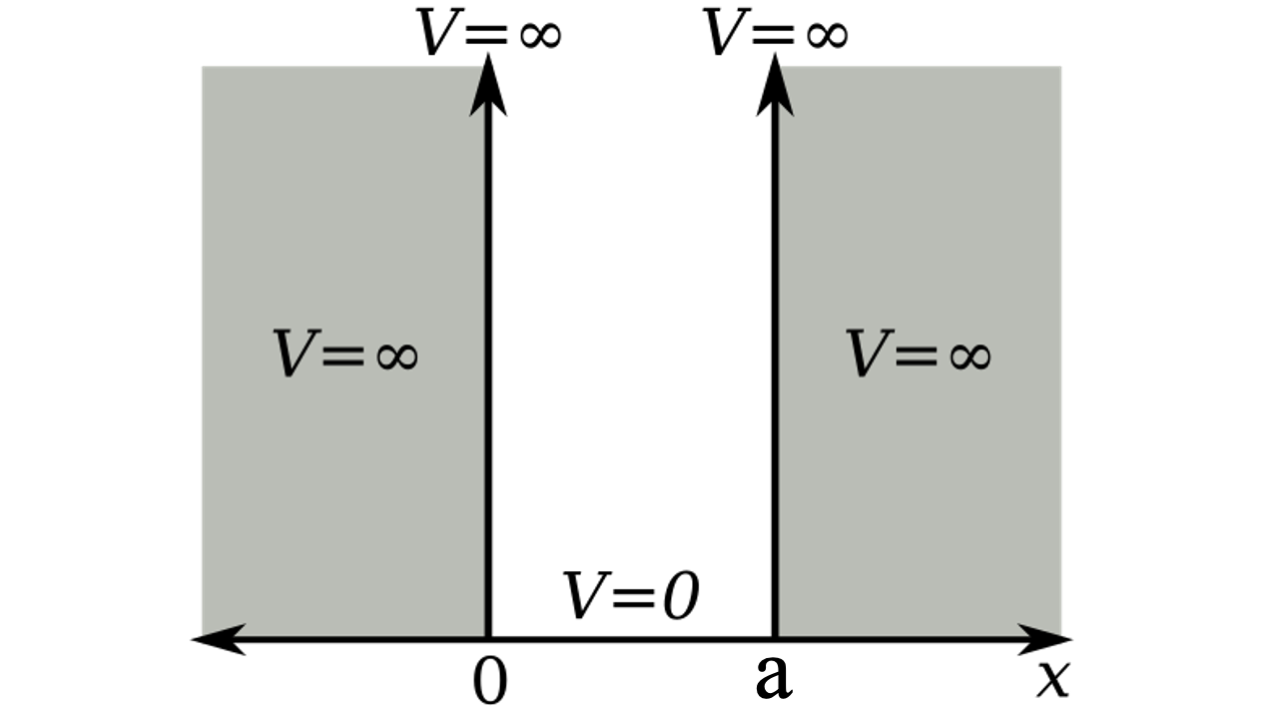
\includegraphics[width=0.5\textwidth]{lab1/images/pIAB.png}
    \caption{Particle in a Box} %reference
    \label{fig:particleInABox}
\end{figure}

\[
  V(x) = \begin{cases}
  0 & 0 < x < a\\
  \infty & \text{elsewhere}
\end{cases}
\]
   
\section{Results}
\subsection{Energy Eigenvalues}
To determine the energy of the quantised states within the potential well, the time-independent one-dimensional Schrödinger equation must be considered:

$$E_n \psi_n (x) = \frac{-\hbar ^{2}}{2m}\frac{\delta^{2}}{\delta x^{2}}\psi_n (x) + V(x)\psi_n (x)$$
where $\hbar$ is the reduced Planck Constant, $m$ is the mass of the particle, $\psi_n (x)$ is the wavefunction, $V(x)$ is the potential, $E_n$ is the energy level and x is the position along the x-axis. 

$V(x)=0$ in the potential well: 

\begin{equation} \label{eq:shrod}
\therefore E_n \psi_n (x) = \frac{-\hbar ^{2}}{2m}\frac{\delta^{2}}{\delta x^{2}}\psi_n (x)
\end{equation}

Substituting $\psi_n (x)$ for its eigenfunction (the derivation for this eigenfunction can be found in Section~\ref{sec:eigenFunction}):
\begin{align*}
E_n \psi_n (x) &= \frac{-\hbar ^{2}}{2m}\frac{\delta^{2}}{\delta x^{2}}\Bigg(\sqrt{\frac{2}{a}}\sin\Big(\frac{n\pi x}{a}\Big)\Bigg)\\
E_n \psi_n (x) &= \frac{-\hbar ^{2}}{2m}\Big(\frac{n\pi}{a}\Big)^{2}\Bigg(\sqrt{\frac{2}{a}}\sin\Big(\frac{n\pi x}{a}\Big)\Bigg)\\
\hspace{-1.2cm}\text{Substituting the eigenfunction for }\psi_n (x)\text{:}\\
E_n \psi_n (x) &= \frac{\hbar ^{2}}{2m}\Big(\frac{n\pi}{a}\Big)^{2}\psi_n (x)\\
E_n &= \frac{\hbar ^{2}}{2m}\Big(\frac{n\pi}{a}\Big)^{2} & \text{where } n \in \mathbb{N}
\end{align*}

The energy eigenvalues for a well of width a=0.1nm is shown in Figure \ref{fig:eigenEnergy} for ($n=1$ to $n=5$)

\begin{figure}[h]
    \centering
    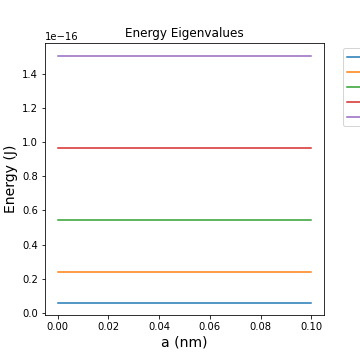
\includegraphics[width=0.4\textwidth]{lab1/images/eigenvaluesEnergy.png}
    \caption{Plot showing the first 5 the discrete energy levels (n=1 to n=5) for a particle confined in a box of length 0.1nm} 
    \label{fig:eigenEnergy}
\end{figure}

The values for the quantised energies can be found in Table \ref{tab:qEnerergy}:

\begin{table}[h!]
\centering
\begin{tabular}{|l|l|l|}
\hline
\textbf{n} & \textbf{Energy (J)} \\ \hline
1 & 6.02467e-18 \\ \hline
2 & 2.40987e-17 \\ \hline
3 & 5.42220e-17 \\ \hline
4 & 9.63946e-17 \\ \hline
5 & 1.50617e-16 \\ \hline
\end{tabular}
%\captionsetup{font = it, labelfont = bf, width=.91\linewidth, justification=centering}
\caption{Table showing the first 5 the discrete energy values (n=1 to n=5) for a particle confined in a box of length 0.1nm}
\label{tab:qEnerergy}
\end{table}

\subsection{Eigenfunctions}\label{sec:eigenFunction}
Equation \ref{eq:shrod} must firstly be rearranged to determine the eigenfunction -- aka the normalised wavefunction:

$$\frac{\delta^{2}}{\delta x^{2}}\psi (x) = \frac{-2m}{\hbar} E \psi (x) = -k^2 \psi (x)$$
$$\frac{\delta^{2}}{\delta x^{2}}\psi (x) + k^2 \psi (x) = 0$$
where $k=\frac{-2m}{\hbar}$

To satisfy this second order homogeneous differential equation, the general equation is given by the following expression:

$$\psi (x) = A \sin(kx) + B \cos(kx)$$

Applying the boundary condition, $\psi (0)$=0:
\begin{align*}
\implies 0 &= A sin(0) + B cos(0)\\
 0 &= B\\
\therefore \psi (kx) &= A sin(kx)
\end{align*}

Applying the boundary condition, $\psi (a)$=0:
\begin{align*}
\hspace{3.5cm} \implies 0 &= A sin(ka)\\
ka &= \pi n & \text{where } n \in \mathbb{N}\\
k &= \frac{\pi n}{a}\\
\therefore \psi_n (x) &= A sin(\frac{\pi n}{a}x)
\end{align*}

The eigenfunction must satisfy the following condition:

$$\int_{ -\infty}^{\infty}\psi_n (x)^{*}\psi_n (x)dx = 1$$
$$\int_{ -\infty}^{0}\psi_n (x)^{*}\psi_n (x)dx +\int_{0}^{a}\psi_n (x)^{*}\psi_n (x)dx + \int_{ a}^{\infty}\psi_n (x)^{*}\psi_n (x)dx= 1$$
\begin{align*}
\int_{ 0}^{a} A^{*} [sin(\frac{\pi n}{a}x)]^{*}A sin(\frac{\pi n}{a}x)dx = 1\\
A^{*}A\int_{ 0}^{a} [sin(\frac{\pi n}{a}x)]^{*}sin(\frac{\pi n}{a}x)dx = 1\\
\left | A \right |^2 \int_{ 0}^{a} sin(\frac{\pi n}{a}x) sin(\frac{\pi n}{a}x)dx = 1\\
\left | A \right |^2 \int_{ 0}^{a} sin^{2}(\frac{\pi n}{a}x)dx = 1\\
\left | A \right |^2 \left[\frac{x}{2}-\frac{asin(\frac{2 \pi nx}{a})}{4 \pi n}\right]_0^a= 1\\
\left | A \right |^2 [(\frac{a}{2}-0)-(0-0)]= 1\\
\left | A \right |^2 \frac{a}{2}= 1\\
\left | A \right | = \sqrt{\frac{2}{a}}
\end{align*}
$$\therefore \psi_n (x) = \sqrt{\frac{2}{a}} sin(\frac{\pi n}{a}x)$$

The normalised wavefunction, $\psi_n (x)$, for $n=1$ to $n=5$ is shown in Figure \ref{fig:normWave}.
\begin{figure}[h]
    \centering
    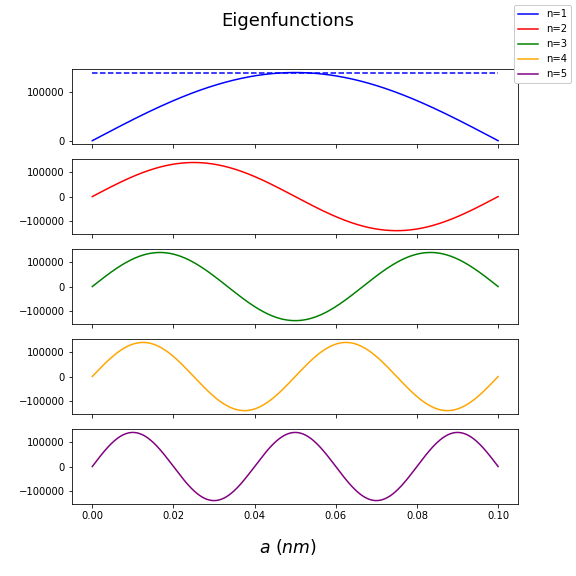
\includegraphics[width=0.6\textwidth]{lab1/images/normalisedWavefunction.png}
    \caption{Plot showing the normalised wavefunctions for (n=1 to n=5) for a particle confined in a box of length 0.1nm}
    \label{fig:normWave}
\end{figure}

Figure \ref{fig:probDens} shows the probability density functions (PDFs), $P_n(x)$, for $n=1$ to $n=5$; where $P_n (x)$, given by:

$$P_n(x) =\psi_n (x)^{*}\psi_n (x) =|\psi_n(x)|^{2} = \Bigg|\sqrt{\frac{2}{a}}\sin\Big(\frac{n\pi x}{a}\Big)\Bigg|^{2}  $$

\begin{figure}[h]
    \centering
    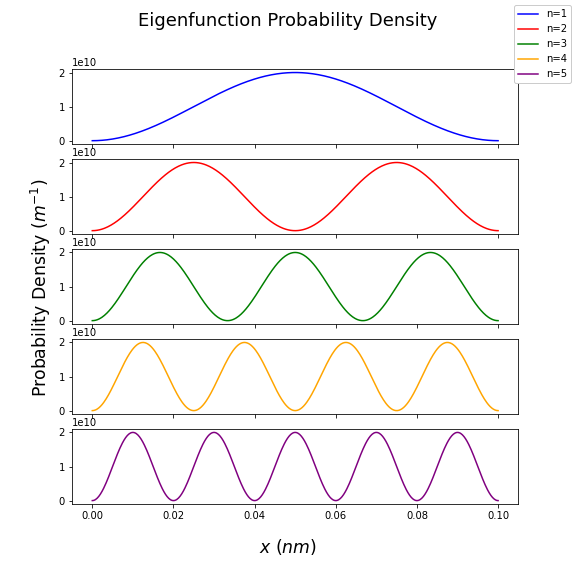
\includegraphics[width=0.6\textwidth]{lab1/images/probabilityDensity.png} %MISSING Y AXIS
    \caption{Plot showing the probability density functions for (n=1 to n=5) for a particle confined in a box of length 0.1nm}
    \label{fig:probDens}
\end{figure}

\subsection{Superposition}

The eigenstates of the system plotted above are stationary. This means that when the system is in one of these eigenstates, all quantum mechanical observables are conserved in time (probability $P=|\Psi(x,t)|^2dx$ is independent of $\phi(t)$, meaning $P=|\psi(x)|^2dx$).

Superpositons of eigenfunctions are not stationary. To observe their non-stationary behaviours, namely, their time evolution we must calculate the superposition state for two states. The wavefunction for one state is given by:

$$\Psi_n (x,t) = \psi_n (x)\phi_n (t)$$
where $\psi_n (x)= \sqrt{\frac{2}{a}} sin(\frac{\pi n}{a}x)$ and $\phi_n (t)= e^{-i \omega t}$

The superposition state is therefore given by:
\begin{equation} \label{eq:superPos}
\Psi_s (x,t) = \psi_n (x)e^{-i \omega_{1} t} + \psi_m (x)e^{-i \omega_{2} t}
\end{equation}

This superposition wavefunction needs to be normalised, i. e.:
$$\int_{ -\infty}^{\infty} A^{*} \Psi_s (x,t)^{*} A\Psi_s (x,t)dx = 1$$
$$\left | A \right |^2 \int_{ -\infty}^{\infty} \Psi_s (x,t)^{*} \Psi_s (x,t)dx = 1$$

Given $\Psi_s (x,t)=0$ for $x<0, x>a$:
$$\left | A \right |^2 \int_{0}^{a} \Psi_s (x,t)^{*} \Psi_s (x,t)dx = 1$$

Substituting Equation \ref{eq:superPos}:
$$\left | A \right |^2 \int_{0}^{a} (\psi_n (x)^{*}e^{i \omega_{1} t} + \psi_m (x)^{*}e^{i \omega_{2} t}) (\psi_n (x)e^{-i \omega_{1} t} + \psi_m (x)e^{-i \omega_{2} t})dx = 1$$
$$\left | A \right |^2 \int_{0}^{a} (\left | \psi_n (x) \right |^2 + \left | \psi_m (x) \right |^2 + \psi_n (x)^{*}\psi_m (x)e^{-i(\omega_{2}- \omega_{1}) t} + \psi_m (x)^{*}\psi_n (x)e^{i(\omega_{2}- \omega_{1}) t})dx = 1$$

In this case $\psi_n (x)$ and $\psi_m (x)$ are completely real;\\
thus, $\psi_n (x)^{*} = \psi_n (x)$ and $\psi_m (x)^{*} = \psi_m (x)$:
$$ \left | A \right |^2 \int_{0}^{a}\left( \left | \psi_n (x) \right |^2 + \left | \psi_m (x) \right |^2 + \psi_m (x)\psi_n (x)(e^{-i(\omega_{2}- \omega_{1})t}+e^{i(\omega_{2}- \omega_{1})t})\right)dx = 1$$

Since $cos(x) = \frac{e^{ix}+e^{-ix}}{2}$:
$$ \left | A \right |^2 \int_{0}^{a}\left( \left | \psi_n (x) \right |^2 + \left | \psi_m (x) \right |^2 + \psi_m (x)\psi_n (x)(2\cos(\omega_{2}- \omega_{1})t)\right)dx = 1$$
$$ \left | A \right |^2 \int_{0}^{a}\left(\frac{2}{a} sin^{2}(\frac{\pi n_1}{a}x)+\frac{2}{a} sin^{2}(\frac{\pi n_2}{a}x)+\frac{4}{a} sin(\frac{\pi n_1}{a}x)sin(\frac{\pi n_2}{a}x)(\cos(\omega_{2}- \omega_{1})t)\right)dx = 1$$
$$...$$
$$\left | A \right |^2 \left( \frac{2}{a}\left(\frac{a}{2}\right) + \frac{2}{a}\left(\frac{a}{2}\right) + \frac{4}{a}\cos(\omega_{2}- \omega_{1})t\int_{0}^{a} sin(\frac{\pi n_1}{a}x)sin(\frac{\pi n_2}{a}x)dx \right)=1$$

$$\left | A \right |^2 \left( 1 + 1 + \frac{4}{a}\cos(\omega_{2}- \omega_{1})t(0) \right)=1$$
$$\left | A \right |^2 = \frac{1}{2}$$
$$\left | A \right | = \sqrt{\frac{2}{a}}$$
$$\therefore \Psi_s (x, t) = \sqrt{\frac{1}{2}} \left( \psi_n (x)e^{-i \omega_{1} t} + \psi_m (x)e^{-i \omega_{2} t}\right)$$

The real part of this superpositioned wavefunction was plotted as shown in Figure \ref{fig:superPosWave}.

\begin{figure}[h]
    \centering
    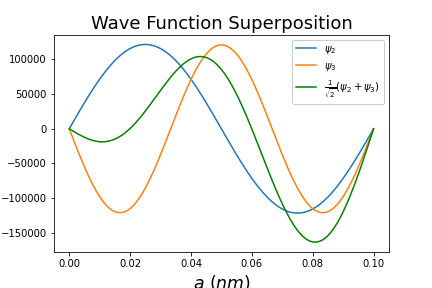
\includegraphics[width=0.65\textwidth]{lab1/images/superpositionWave.png}
    \caption{Plot showing the two eigenstates, $\psi_2 (x)$ and $\psi_3 (x)$, and the superposition of both eigenstates for a particle confined in a box of length 0.1nm at time \textbf{t=1}}
    \label{fig:superPosWave}
\end{figure}

The probability distribution of the new wavefunction $\Psi_s(x,t)$ was then calculated and plotted at several different times to see how it evolves in time, shown in Figure \ref{fig:superPosPDF}.

$$P_s(x, t) = A^{*} \Psi_s (x, t)^{*} A\Psi_s (x, t)$$
$$P_s(x) = \left | A \right |^2 \Psi_s (x,t)^{*} \Psi_s (x,t)$$
$$P_s(x) = 0.5 (\psi_n (x)^{*}e^{i \omega_{1} t} + \psi_m (x)^{*}e^{i \omega_{2} t}) (\psi_n (x)e^{-i \omega_{1} t} + \psi_m (x)e^{-i \omega_{2} t})$$
$$P_s(x) = 0.5 (\left | \psi_n (x) \right |^2 + \left | \psi_m (x) \right |^2 + \psi_n (x)^{*}\psi_m (x)e^{-i(\omega_{2}- \omega_{1}) t} + \psi_m (x)^{*}\psi_n (x)e^{i(\omega_{2}- \omega_{1}) t})$$

As stated earlier $\psi_n (x)=\psi_n (x^{*})$ and $\psi_m (x)=\psi_m (x^{*})$:
$$\therefore P_s(x) =  0.5 (\left | \psi_n (x) \right |^2 + \left | \psi_m (x) \right |^2 + \psi_n (x)\psi_m (x)e^{-i(\omega_{2}- \omega_{1}) t} + \psi_m (x)\psi_n (x)e^{i(\omega_{2}- \omega_{1}) t})$$
$$P_s(x) = 0.5 (\left | \psi_n (x) \right |^2 + \left | \psi_m (x) \right |^2 + \psi_n (x)\psi_m (x)(e^{-i(\omega_{2}- \omega_{1}) t} + e^{i(\omega_{2}- \omega_{1}) t}))$$

Since $\cos(x)=\frac{e^{-ix}+e^{ix}}{2}$:
$$P_s(x) = 0.5 (\left | \psi_n (x) \right |^2 + \left | \psi_m (x) \right |^2 + \psi_n (x)\psi_m (x)(2\cos\omega t))$$
$$P_s(x) = 0.5 \left | \psi_n (x) \right |^2 + 0.5\left | \psi_m (x) \right |^2 + \psi_n (x)\psi_m (x)\cos\omega t$$

\begin{figure}[h]
    \centering
    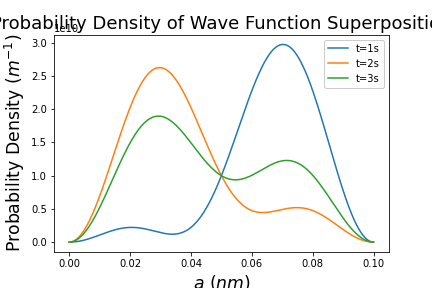
\includegraphics[width=0.75\textwidth]{lab1/images/superpositionPDF.png}
    \caption{Probability density function for the superimposed state, $\Psi_s (x,t)$, plotted at various times}
    \label{fig:superPosPDF}
\end{figure}

\section{Comparison of Results with Theory}

The results from this lab is entirely based on theory so there are no discrepancies of the results with theory.

To ensure this is true 

When calculating $E_n$ for $n=1,2,3,4,5$ it is clear to see that the ratio of $\frac{E_n}{E_1}$ is always equal to $n^{2}$
Substituting $n=1$:
$$E_1 = \frac{\hbar ^{2}\pi^{2}}{2ma^{2}}$$

\begin{equation}%\label{eq:energySpacing}
\implies E_n =  n^{2}E_1
\end{equation}
The energy levels must therefore become more sparse as $n$ increases, which can be seen in Figure \ref{fig:eigenEnergy}

All of the wave functions are 0 at each wall which means that the boundary conditions were always satisfied.

The peak wavefunctions $\approx \sqrt{2/L}$ and the peak probability is no higher than $2/L$.

The area under the probability density functions must always be equal to 1. To verify this the trap function was used.

Talk about plotting the real part and leaving out the imaginary part?


Also, the maximum of each wavefunction reaches the theoretical limit without surpassing it. The limit is:

$$ \text{Maximum}(|\Psi_n(x)|) = \sqrt{\frac{2}{L}} = \sqrt{\frac{2}{0.1e-9}} \approx  141421 $$

This is the necessary amplitude of the wave to achieve a normalised wavefunction.
The maximum of the wavefunction was found to be $141421$, \textbf{indicating that the plot is accurate. The same can be seen for Figure 1.3, where the theoretical limit is}:

$$ \text{Maximum}(|\Psi_n(x)|^{2}) = \frac{2}{L} = \frac{2}{0.1 \times 10^{-9}} = 2e^{10} $$

Again the peak value of the PDF was found to be $2e10$, \textbf{confirming the accuracy}.

\textbf{To confirm the PDF matches the theory and is being plotted correctly, it has to always satisfy the normalisation condition $\int_{0}^{a} |\Psi_s(x,t)|^{2} \,\delta x = 1$. By using the \textit{'trapz'} function to calculate an approximate area under the curve using the trapezium rule, it was found that the area ranged from 0.999998 to 1.000003 as $t$ progressed. The source of error comes from the intrinsic error of the trapezium rule and how the trapeziums cannot ever have infinitesimally small width}

Finally, by visual inspection we can see that the superposition is correct for all values of $t$. By choosing a location where one of $|\Psi_n(x)|$ or $|\Psi_m(x)| = 0$, we can see that the height of $|\Psi_s(x)|$ is $\frac{1}{\sqrt{2}}$ that of the non-zero wavefunction, thus confirming the superposition of the two is being calculated correctly. 

\section{Discussion}
\textbf{Question 1:}
After creating the energy-level diagram for up to $n=5$, create a code that finds the wavelengths of the photons emitted for all transitions beginning at state $n=3$ or less and ending at a lower energy state.

The wavelength was found using the following equation:

\[\lambda = \frac{hc}{\Delta E}\]
where $\lambda$ is the wavelength of the photon, $h$ is Planks constant, $c$ is the speed of light and $\Delta E$ is the difference in eigen energies.

\begin{listing}
\begin{minted}[
frame=lines,
framesep=2mm,
baselinestretch=1.2,
bgcolor=LightGray,
fontsize=\footnotesize,
linenos
]{python}

def wavelength(E):
    l = const.Planck*const.c/E
    return l

#Transition n=3 to n=2
print("n=3 to n=2 photon wavelength: ", 
      wavelength(Eigen_energies[2]-Eigen_energies[1]),"m")
#Transition n=3 to n=1
print("n=3 to n=1 photon wavelength: ", 
      wavelength(Eigen_energies[2]-Eigen_energies[0]),"m")
#Transition n=2 to n=1
print("n=2 to n=1 photon wavelength: ", 
      wavelength(Eigen_energies[1]-Eigen_energies[0]),"m")
\end{minted}
\end{listing}

\begin{lstlisting}[frame=single,style=base,backgroundcolor=\color{black}, basicstyle=\small]
@>>> n=3 to n=2 photon wavelength:  6.594375173013399e-09 m
>>> n=3 to n=1 photon wavelength:  4.1214844831333745e-09 m
>>> n=2 to n=1 photon wavelength:  1.0990625288355668e-08 m@
\end{lstlisting}


\section{Conclusions}

\begin{itemize}
    \item Visualise the energy levels of a confined particle as well as the behaviour of its quantum wavefunction,
    \item Obtain deeper understanding and visualise the nature of qunatum superposition.
\end{itemize}

\renewcommand{\chaptername}{March 8th: Lab}
\chapter{Qubits and Quantum Circuits}
%rotate the STATE? or QUBIT?
%centre captions

Conventionally, information is stored in bits, as a series of 0s and 1s. However, in quantum computing `quantum bits', or simply `qubits', are used. These obey the rules of quantum mechanics and allow for information to be processed in new and different ways.

In order to manipulate these qubits (i.e. change them between quantum states) `quantum gates' can be applied to build a 'quantum circuit'. A quantum circuit is a computational routine consisting of coherent quantum operations on quantum data, such as qubits, and concurrent real-time classical computation. It is an ordered sequence of quantum gates, measurements and resets, all of which may be conditioned on and use data from the real-time classical computation.

\section{Objectives}
The purpose of this lab is to investigate quantum bits and quantum circuits using IBM's `qiskit`. Thus, the following objectives were pursued:
\begin{itemize}
    \item Become familiar with `qiskit'
    \item Implement quantum gates and visualise the state of a qubit through the Bloch sphere
    \item Obtain deeper understanding of quantum operations and quantum circuits basics
\end{itemize}

\section{Methods}
Quantum circuits were implemented and visualised using python in Jupyter Notebook -- a web-based interactive computational environment for programming languages. Specifically, a library named `qiskit' was used -- an open-source software development kit for working with quantum computers. It provides tools for creating quantum programs and for running them on simulators on a local computer. The Aer simulator was used; this provides high-performance quantum computing simulators with realistic noise models locally, and visualization allows you to see what you states look like

To evaluate the rigidity of the analytical predictions from qiskit, the circuits were built on protoype quantum devices provided by IBM Quantum. `The IBM Quantum Composer' is an online platform allowing public access to remote quantum computing services.

%Reference screenshots of code

\section{Results}
Qubits can be represented by 2D vectors, their states are limited to the form:

$$ |q\rangle = \cos{\tfrac{\theta}{2}}|0\rangle + e^{i\phi}\sin{\tfrac{\theta}{2}}|1\rangle $$
where $\theta$ and $\phi$ are real numbers. 

This state can be visualized using a `Bloch Sphere' (a geometrical representation of a two-level qubit) and quantum gates can be used to manipulate the state. An important feature of quantum circuits is that quantum gates are always reversible. These reversible gates can be represented as matrices, and as rotations around the Bloch sphere.

In this lab report, Pauli gates, the Hadamard gate and some Multi-qubit gates are analysed in detail.

\subsection{The Pauli Gates}
Pauli matrices can represent some commonly used quantum gates. 

\subsubsection{The X Gate}
The X gate is represented by the Pauli-X matrix:

$$ X = \begin{bmatrix} 0 & 1 \\ 1 & 0 \end{bmatrix} = |0\rangle\langle1| + |1\rangle\langle0| $$

A circuit was created to determine the effect an X gate has on a qubit. A qubit was initialised in state $|0\rangle$ and was passed through an X gate, the circuit diagram of which is shown in Figure \ref{fig:xGate}.

\begin{figure}[h]
    \centering
    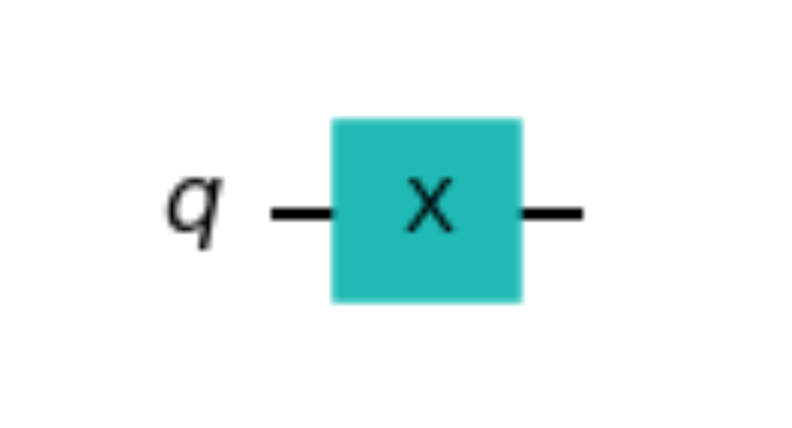
\includegraphics[width=0.3\textwidth]{lab2/images/xGate.png}
    \caption{Circuit diagram of a Pauli-X gate} 
    \label{fig:xGate}
\end{figure}

From the mathematics, it is clear that applying an X gate switches the amplitudes of the states $|0\rangle$ and $|1\rangle$:

$$ X|0\rangle = \begin{bmatrix} 0 & 1 \\ 1 & 0 \end{bmatrix}\begin{bmatrix} 1 \\ 0 \end{bmatrix} = \begin{bmatrix} 0 \\ 1 \end{bmatrix} = |1\rangle \quad\quad\quad\quad
X|1\rangle = \begin{bmatrix} 0 & 1 \\ 1 & 0 \end{bmatrix}\begin{bmatrix} 0 \\ 1 \end{bmatrix} = \begin{bmatrix} 1 \\ 0 \end{bmatrix} = |0\rangle$$

%DEMONSTRATED
The circuit in Figure \ref{fig:xGate} was implemented in X and the states were obeserved using a Bloch sphere. Figure \ref{fig:bSphereXGate} shows the X gate performs a rotation by $\pi$ around x-axis of the Bloch sphere (the qubit switched to state $|1\rangle$ after being initialised in state~$|0\rangle$).

\begin{figure}[h]
    \centering
    \begin{subfigure}[h]{0.33\textwidth}
        \centering
        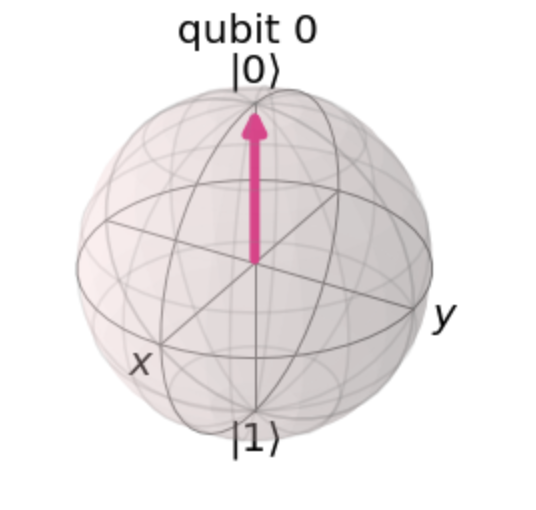
\includegraphics[width=\textwidth]{lab2/images/bSphX1.png}
        \caption{}
        \label{fig:bSphX1}
    \end{subfigure}
    \hspace{0.2\textwidth}
    \begin{subfigure}[h]{0.33\textwidth}
        \centering
        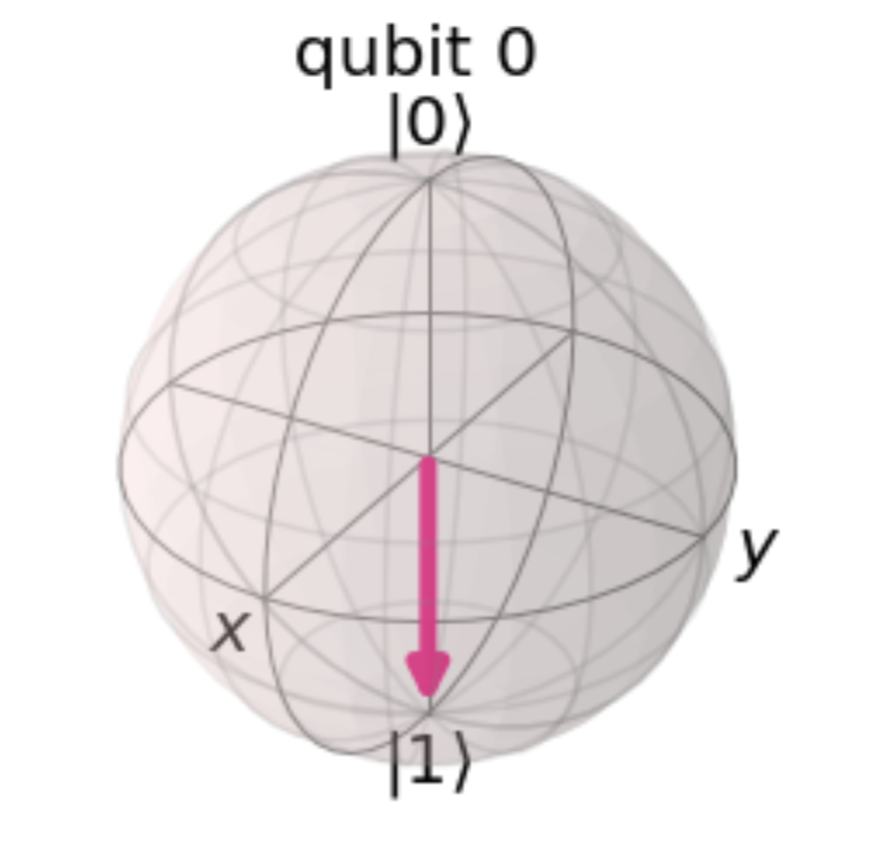
\includegraphics[width=\textwidth]{lab2/images/bSphX2.png}
        \caption{}
        \label{fig:bSphX2}
    \end{subfigure}
    \caption{Bloch sphere showing a) the state of the initialised qubit and b) the state of the qubit after being passed through a Pauli-X gate} 
    \label{fig:bSphereXGate}
\end{figure}

\subsubsection{The Y and Z gates}

Similar to the X gate, the Y and Z Pauli matrices can represent the Y and Z gates in our quantum circuits. These gates perform rotations by $\pi$ around the y and z-axis of the Bloch sphere, respectively.

$$ Y = \begin{bmatrix} 0 & -i \\ i & 0 \end{bmatrix} = -i|0\rangle\langle1| + i|1\rangle\langle0| $$

$$ Z = \begin{bmatrix} 1 & 0 \\ 0 & -1 \end{bmatrix} = |0\rangle\langle0| - |1\rangle\langle1| $$

A circuit was created with an X and Y gate in series, as shown in Figure \ref{fig:xyGateDiagram}.

\begin{figure}[h]
    \centering
    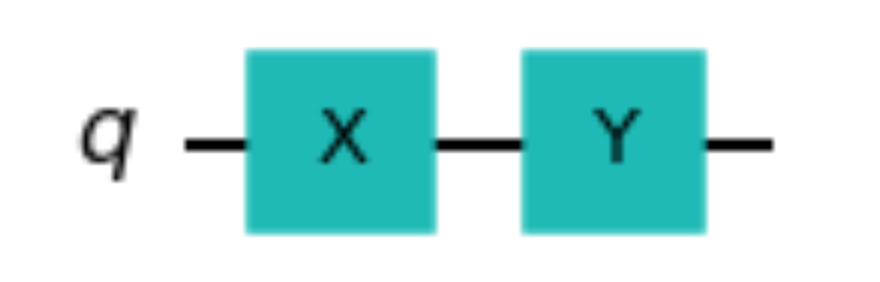
\includegraphics[width=0.3\textwidth]{lab2/images/xyGate.png}
    \caption{Circuit diagram of Pauli-X gate followed by a Pauli-Y gate in series} 
    \label{fig:xyGateDiagram}
\end{figure}

The resultant state was observed through the use of a Bloch sphere. After passing through circuit described in Figure \ref{fig:xyGateDiagram}, the qubit was found to be in state $|0\rangle$ -- seemingly unchanged from its initialised state -- as seen in Figure \ref{fig:xyGateBloc}.

\begin{figure}[h]
    \centering
    \begin{subfigure}[h]{0.33\textwidth}
        \centering
        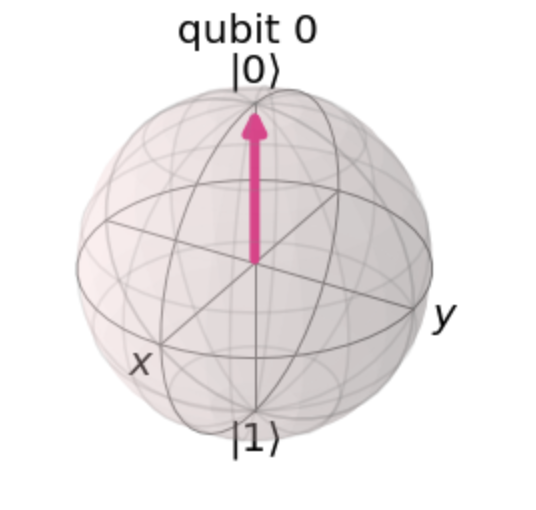
\includegraphics[width=\textwidth]{lab2/images/bSphX1.png}
        \caption{}
        \label{fig:bSphXY1}
    \end{subfigure}
    \hspace{0.2\textwidth}
    \begin{subfigure}[h]{0.33\textwidth}
        \centering
        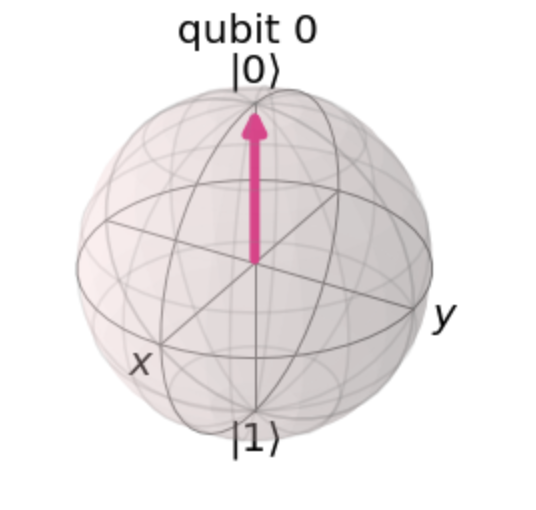
\includegraphics[width=\textwidth]{lab2/images/bSphX1.png}
        \caption{}
        \label{fig:bSphXY2}
    \end{subfigure}
    \caption{Bloch sphere showing a) the state of the initialised qubit and b) the state of the qubit after being passed through a Pauli-X gate and a Pauli-Y gate} 
    \label{fig:xyGateBloc}
\end{figure}

%Need fixed
The explanation for this is as follows:
\begin{enumerate}
    \item The qubit was initialised in state $|0\rangle$
    \item The X gate rotated this state by $\pi$ around the x-axis
    \begin{enumerate}
        \item resulting with a qubit in state $|1\rangle$
    \end{enumerate}
    \item The Y gate then rotated this qubit by $\pi$ around the y-axis
    \begin{enumerate}
        \item resulting in the qubit being in state~$|0\rangle$
    \end{enumerate} 
\end{enumerate}

\subsection{The Hadamard Gate}
The Hadamard gate (H gate) is a fundamental quantum gate, represented by the following matrix:

$$ H = \tfrac{1}{\sqrt{2}}\begin{bmatrix} 1 & 1 \\ 1 & -1 \end{bmatrix} $$

It allows states to occupy a superposition of $|0\rangle$ and $|1\rangle$:

$$ H|0\rangle = \tfrac{1}{\sqrt{2}}\begin{bmatrix} 1 & 1 \\ 1 & -1 \end{bmatrix}\begin{bmatrix} 1 \\ 0 \end{bmatrix} = \tfrac{1}{\sqrt{2}} \begin{bmatrix} 1 \\ 1 \end{bmatrix}= |+\rangle 
\quad \quad \quad \quad 
H|1\rangle = \tfrac{1}{\sqrt{2}}\begin{bmatrix} 1 & 1 \\ 1 & -1 \end{bmatrix}\begin{bmatrix} 0 \\ 1 \end{bmatrix} = \tfrac{1}{\sqrt{2}} \begin{bmatrix} 1 \\ -1 \end{bmatrix}= |-\rangle $$

The H gate can transform the state of the qubit between the X and Z bases. It essentially performs a rotation around the Bloch vector `[1,0,1]' (the line between the x and z-axis).

Applying the sequence of gates: HZH, to any qubit state is equivalent to applying a single X-gate, shown mathematically below.

$$ H = \tfrac{1}{\sqrt{2}}\begin{bmatrix} 1 & 1 \\ 1 & -1 \end{bmatrix} \quad\quad  Z = \begin{bmatrix} 1 & 0 \\ 0 & -1 \end{bmatrix} \quad\quad  X = \begin{bmatrix} 0 & 1 \\ 1 & 0 \end{bmatrix} $$

\begin{equation*} 
\begin{split}
HZH & = \tfrac{1}{\sqrt{2}}\begin{bmatrix} 1 & 1 \\ 1 & -1 \end{bmatrix} \begin{bmatrix} 1 & 0 \\ 0 & -1 \end{bmatrix}\tfrac{1}{\sqrt{2}}\begin{bmatrix} 1 & 1 \\ 1 & -1 \end{bmatrix} \\
HZH & = \tfrac{1}{\sqrt{2}}\tfrac{1}{\sqrt{2}}\begin{bmatrix} 1 & 1 \\ 1 & -1 \end{bmatrix} \begin{bmatrix} 1 & 0 \\ 0 & -1 \end{bmatrix}\begin{bmatrix} 1 & 1 \\ 1 & -1 \end{bmatrix} \\
HZH & = \tfrac{1}{2}\begin{bmatrix} 1 & -1 \\ 1 & 1 \end{bmatrix}\begin{bmatrix} 1 & 1 \\ 1 & -1 \end{bmatrix}\\
HZH & = \tfrac{1}{2}\begin{bmatrix} 0 & 2 \\ 2 & 0 \end{bmatrix} \\
HZH & = \begin{bmatrix} 0 & 1 \\ 1 & 0 \end{bmatrix} \\
HZH & = X
\end{split}
\end{equation*}

The following circuit was written to verify this.

\begin{figure}[h]
    \centering
    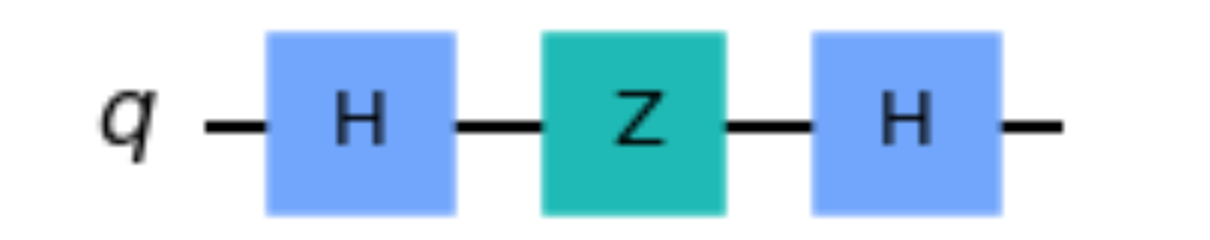
\includegraphics[width=0.4\textwidth]{lab2/images/hzhCircuit.png}
    \caption{Circuit diagram of a Hadamard gate, followed by a Pauli-Z gate, followed by another Hadamard gate in series} 
    \label{fig:hzhCircuit}
\end{figure}

Figure \ref{fig:bSphereHZHGate} shows the resultant state of the qubit after being passed through the circuit shown in Figure \ref{fig:hzhCircuit}.

\begin{figure}[h]
    \centering
    \begin{subfigure}[h]{0.24\textwidth}
        \centering
        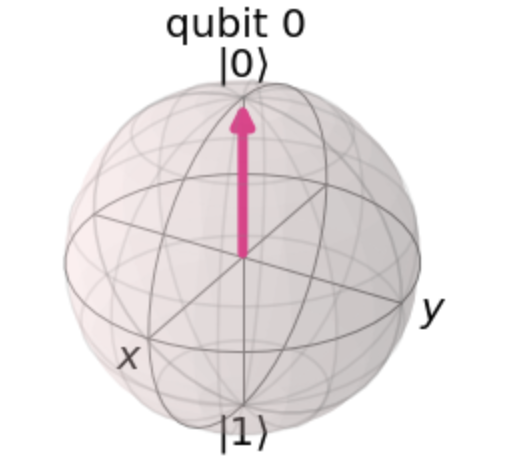
\includegraphics[width=\textwidth]{lab2/images/hzhGate1.png}
        \caption{Initial state}
        \label{fig:hzhGate1}
    \end{subfigure}
    \hfill
    \begin{subfigure}[h]{0.24\textwidth}
        \centering
        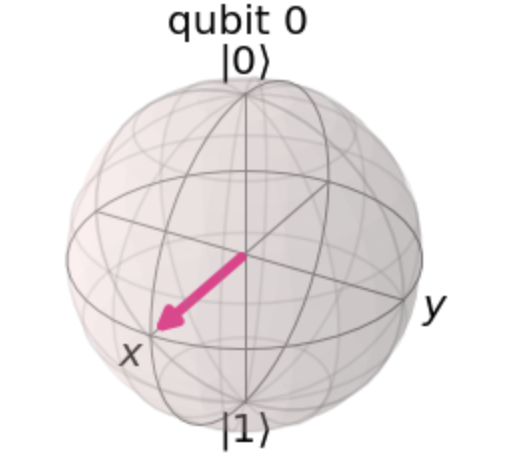
\includegraphics[width=\textwidth]{lab2/images/hzhGate2.png}
        \caption{After H gate}
        \label{fig:hzhGate2}
    \end{subfigure}
        \begin{subfigure}[h]{0.24\textwidth}
        \centering
        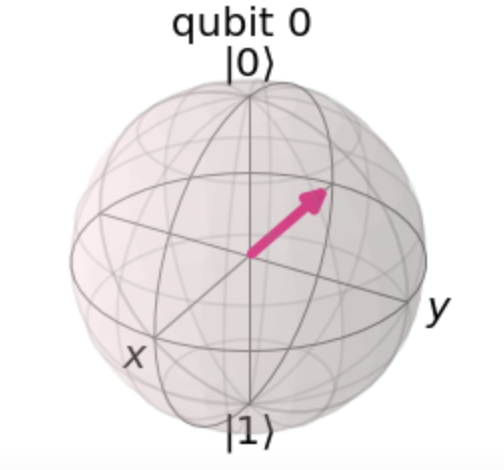
\includegraphics[width=\textwidth]{lab2/images/hzhGate3.png}
        \caption{After Z gate}
        \label{fig:hzhGate3}
    \end{subfigure}
        \begin{subfigure}[h]{0.24\textwidth}
        \centering
        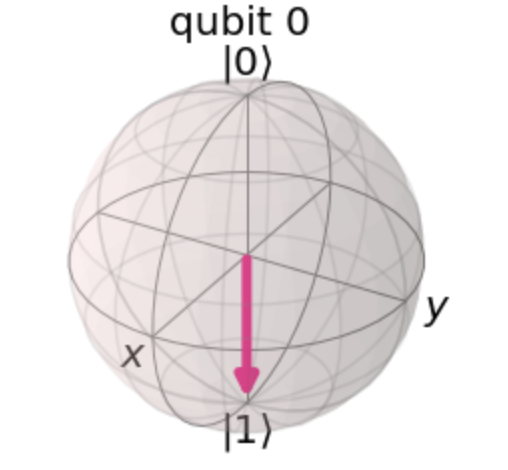
\includegraphics[width=\textwidth]{lab2/images/hzhGate4.png}
        \caption{After H gate}
        \label{fig:hzhGate4}
    \end{subfigure}
    \caption{Bloch sphere showing the state of the qubit after each gate is applied} 
    \label{fig:bSphereHZHGate}
\end{figure}

%FIX?
It is clear upon comparing the initial state (Figure \ref{fig:hzhGate1}) to the final state (Figure \ref{fig:hzhGate4}) that applying the sequence of gates: HZH has an identical effect to applying a single X gate (see Figure \ref{fig:xyGateBloc}).

\subsection{Multi-Qubit Gates}

how to represent the state of a qubit and how to alter those using quantum gates

\subsubsection{The CNOT Gate}
An important two-qubit gate is the CNOT gate. This gate is a conditional gate that performs an X gate on the second qubit (target), if the state of the first qubit (control) is  $|1\rangle$. Table \ref{tab:cNotTruth} shows the truth table for a CNOT gate.

\begin{table}[]
\centering
\begin{tabular}{cccc}
\multicolumn{2}{c}{Input}                         & \multicolumn{2}{c}{Output}   \\ 
\multicolumn{1}{c|}{q1} & \multicolumn{1}{c||}{q2} & \multicolumn{1}{c|}{q1} & q2 \\ \hline\hline
\multicolumn{1}{c|}{0}  & \multicolumn{1}{c||}{0}  & \multicolumn{1}{c|}{0}  & 0  \\ \hline
\multicolumn{1}{c|}{0}  & \multicolumn{1}{c||}{1}  & \multicolumn{1}{c|}{0}  & 1  \\ \hline
\multicolumn{1}{c|}{1}  & \multicolumn{1}{c||}{0}  & \multicolumn{1}{c|}{1}  & 1  \\ \hline
\multicolumn{1}{c|}{1}  & \multicolumn{1}{c||}{1}  & \multicolumn{1}{c|}{1}  & 0 
\end{tabular}
\label{tab:cNotTruth}
\caption{Truth table for CNOT gate}
\end{table}


%q\_1 as the control and q\_2 as the target


A 2-qubit quantum circuit was created, where the 2 qubits are entangled and the output was measured. The circuit diagram is shown in Figure \ref{fig:entangleMeasure}

\begin{figure}[h]
    \centering
    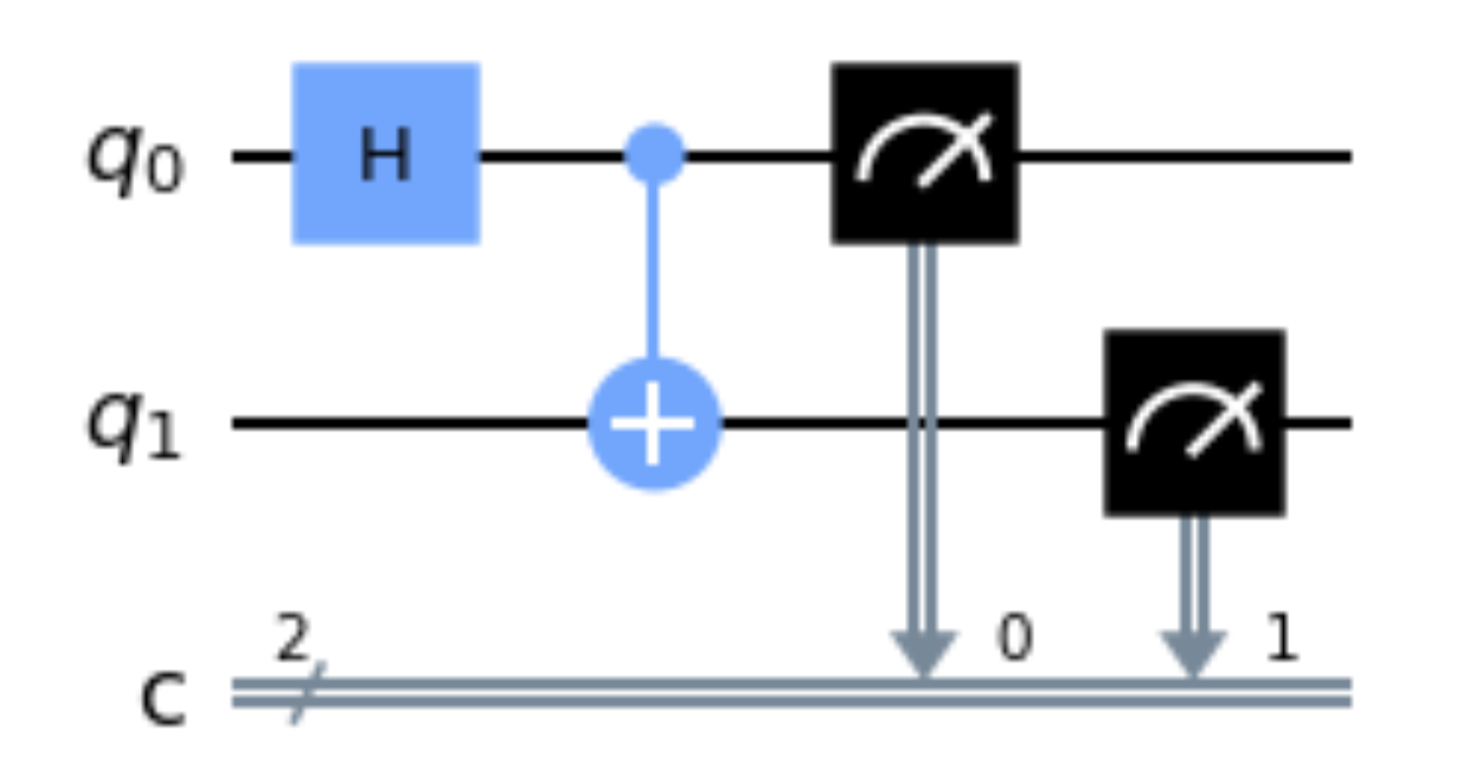
\includegraphics[width=0.4\textwidth]{lab2/images/entangleMeasure.png}
    \caption{entangleMeasure} 
    \label{fig:entangleMeasure}
\end{figure}

So both are initialised as 0. H puts the top in superposition, meaning it is 50\% between 0 and 1. Then when its used as a control bit, its kinda halfway between 0 and 1 meaning half the time it will be a 1 switching the second bit to a 1, then the other half it will be 0 meaning the second qubit will stay 0. As a result, we would expect two possible results from this circuit. Half of the time its 00 and the other half itll be 11. This was circuit was simulated and the results can be found in Figure \ref{fig:qiskitHistogram}.

\begin{figure}[h]
    \centering
    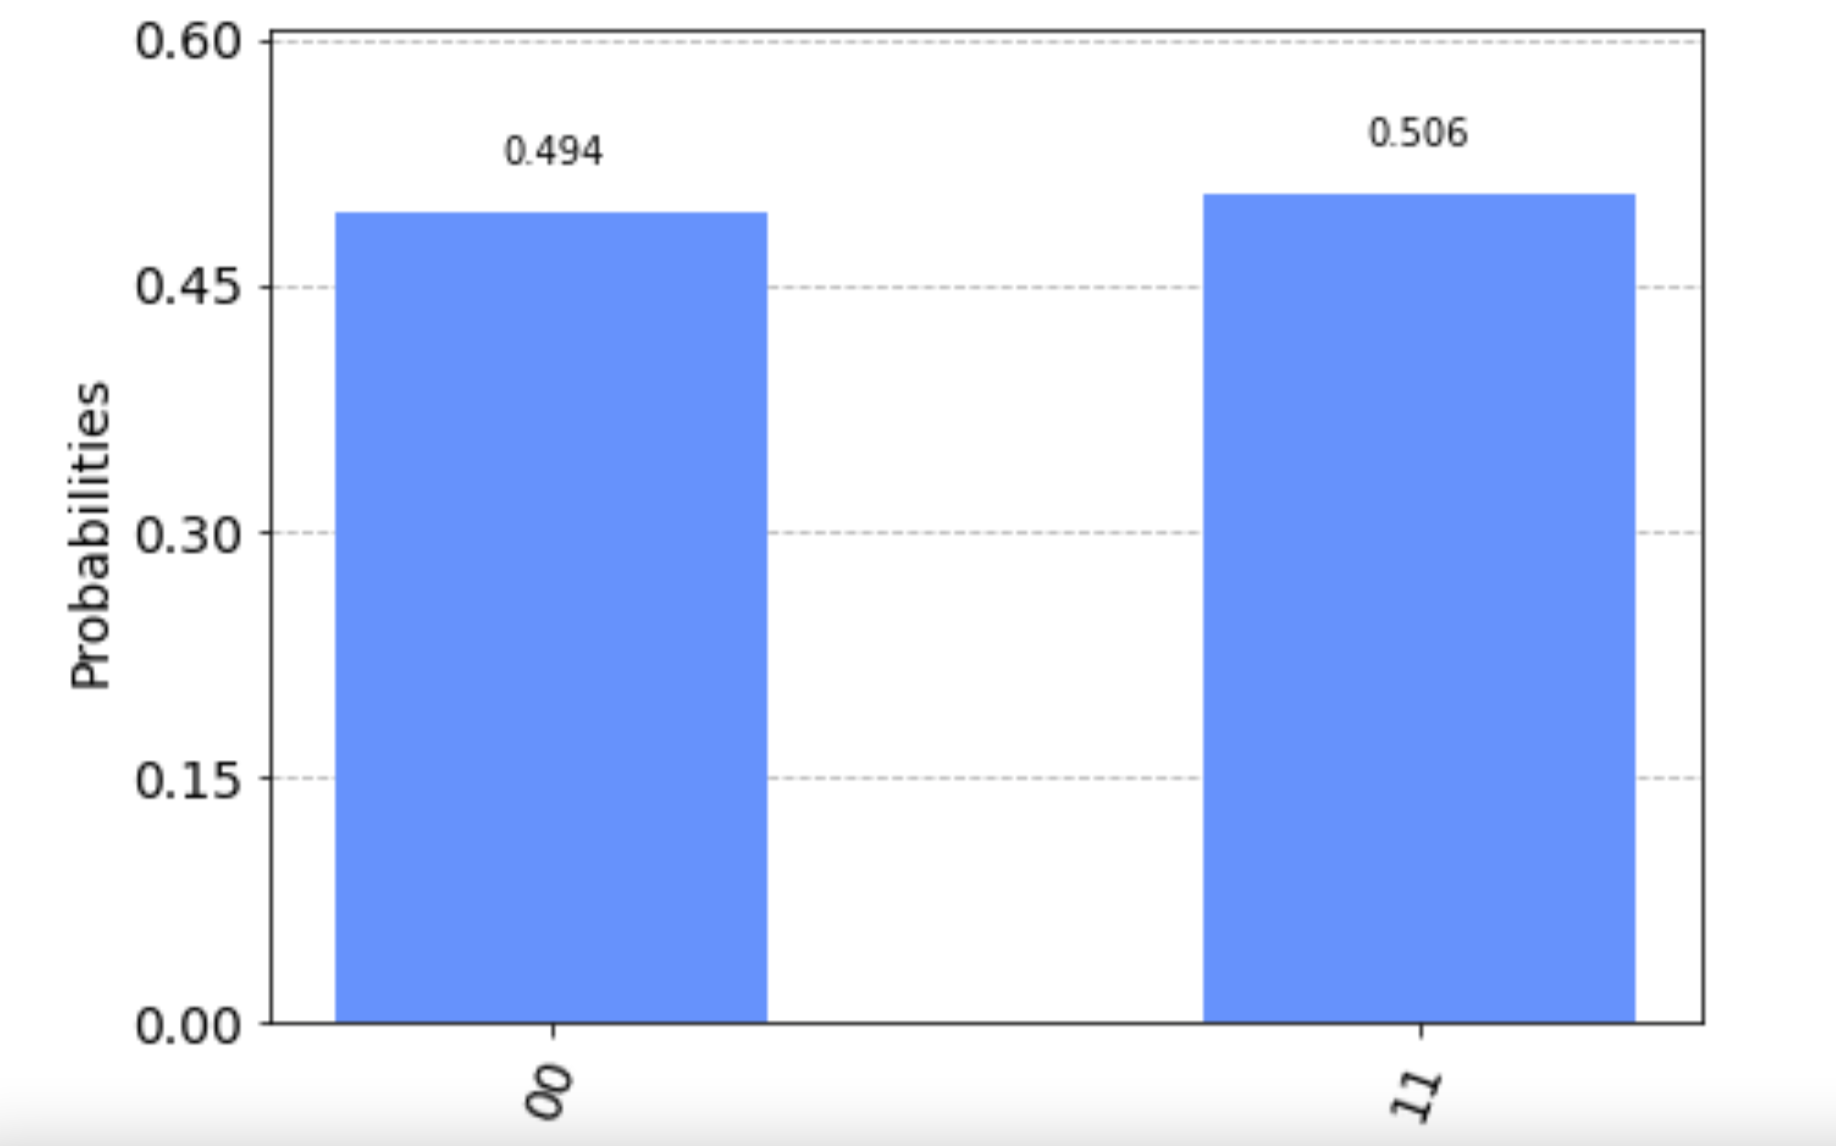
\includegraphics[width=0.75\textwidth]{lab2/images/qiskitHistogram.png}
    \caption{qiskitHistogram} 
    \label{fig:qiskitHistogram}
\end{figure} 

The results show that two 00 and 11 came up which made sense,  however it was not a 50/50 split as expected. This is discussed further in Section \ref{sec:discussion}. To determine a more real response IBMs quantum computer was used. The results can be seen in Figure \ref{fig:ibmHistogram}. Again, there was not a co

\begin{figure}[h]
    \centering
    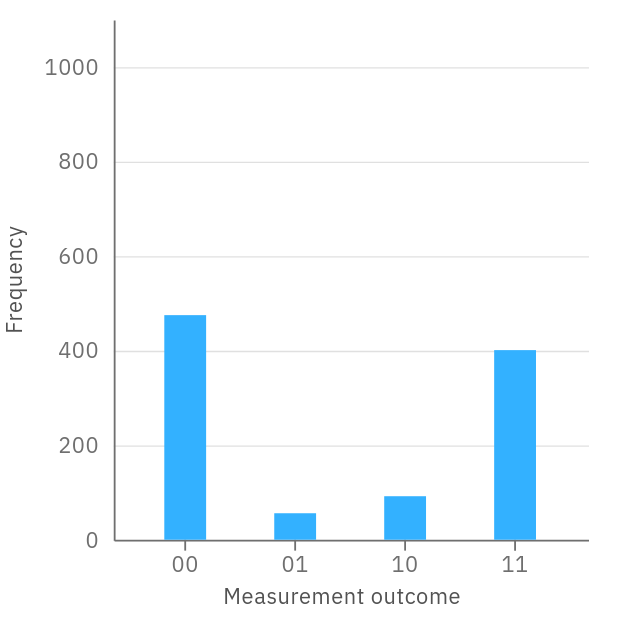
\includegraphics[width=0.4\textwidth]{lab2/images/ibmHistogram.png}
    \caption{qiskitHistogram} 
    \label{fig:ibmHistogram}
\end{figure} 

\section{Comparison of results with theory}
\section{Discussion} \label{sec:discussion}
\textbf{Question 1:}

Initialise a qubit, and apply the X gate to it. Confirm your result by drawing the circuit and visualing the flipped state using the Block sphere (use/copy and paste the examples above wherever appropriate).


\textbf{Question 2:}
Apply the x and y gates to the qubit above and draw it on your screen.

To be frank. That is not a question.

\textbf{Question 3:}
Show mathematically that applying the sequence of gates: HZH, to any qubit state is equivalent to applying an X gate. Then, write a circuit that will show this (you can check each step/rotation, by ploting the new state on the Bloch Sphere each time.


\textbf{Question 4:}
Build a 2-qubit quantum circuit where the 2 qubits are entangled and measure the output. Does this agree with the mathematical prediction? If not, why would you say that is so

\textbf{Question 5:}
Use IBM composer and compare its results to what you obtained above. Are they different? How so? Is there anything you can do to make the results come closer to the mathematica expectation?

\section{Conclusions}

\renewcommand{\chaptername}{March 15th: Lab}
\chapter{Quantum Teleportation}
In quantum teleportation, the properties of quantum entanglement are used to send a qubit between observers without physically moving the involved qubit. The qubits themselves are not really teleported, but the state of one qubit is destroyed on one side and extracted on the other side, so the information that the state encodes is communicated. The process is not instantaneous, because information must be communicated classically between observers as part of the process. The usefulness of quantum teleportation lies in its ability to send quantum information arbitrarily far distances without exposing quantum states to thermal decoherence from the environment or other adverse effects.

This may sound a bit like science fiction, but quantum teleportation can in principle be used to actually teleport macroscopic objects (in the sense that two objects in exactly the same quantum state are identical). However, the number of entangled states necessary to accomplish this is well outside anything physically achievable, since maintaining such a massive number of entangled states without decohering is a difficult problem.

\section{Objectives}

\begin{itemize}
    \item Implement a quantum algorithm
    \item Understand the principles on quantum teleportation and how it can be implemented/applied
\end{itemize}

\section{Methods}

The following qubit state  $|\Psi \rangle = \alpha |0 \rangle + \beta |1 \rangle$ needs to be transferred. This entails passing on information about $\alpha$ and $\beta$. There exists a theorem in quantum mechanics which states that you cannot simply make an exact copy of an unknown quantum state, known as the no-cloning theorem. As a result a copy of  $|\Psi \rangle$ cannot simply be generated (classical states can be copied, not superpositions).

By taking advantage of two classical bits and an entangled qubit pair, the state $|\Psi \rangle$ can be transferred.

This is called teleportation because, at the end, the state $|\Psi \rangle$ will be with the end user and not with the sendee anymore.

\subsection{Teleportation Protocol}
The following steps were followed to create an entanglement protocol and to perform quantum teleportation.

\begin{enumerate}
    \item Use a third party entangled qubit pair
    \item Alice should then perform some operations on her qubit
    \item Then send the results to Bob over a classical communication channel
    \item Bob then performs some operations on his end to receive Alice’s qubit
\end{enumerate}

\section{Results}

The final circuit is shown in Figure \ref{fig:teleportCircuit}
\begin{figure}[h]
    \centering
    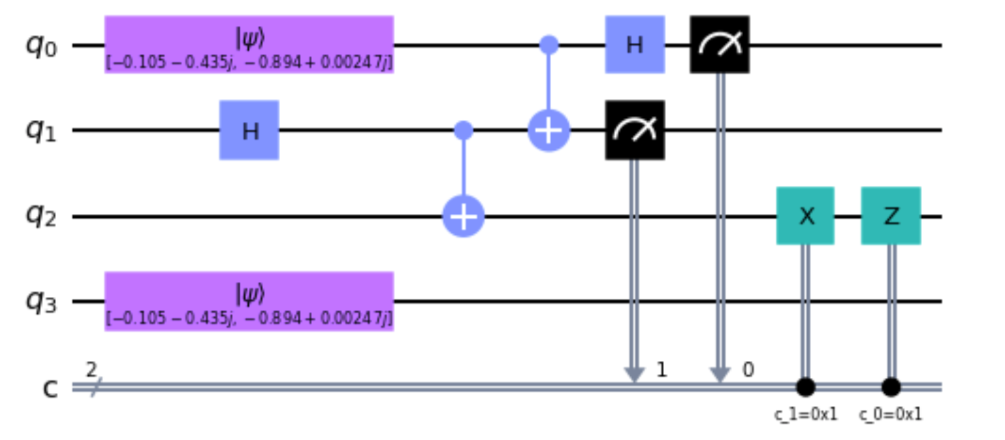
\includegraphics[width=0.6\textwidth]{lab3/teleportCircuit.png}
    \caption{teleportCircuit}
    \label{fig:teleportCircuit}
\end{figure}

\subsubsection{Step 1}
My work

\subsubsection{Step 2}
My work

\subsubsection{Step 3}
My work

\subsubsection{Step 4}
My work

The result from this circuit was observed using Bloch Sphere representation, as seen in Figure \ref{fig:teleportBloch}
\begin{figure}[h]
    \centering
    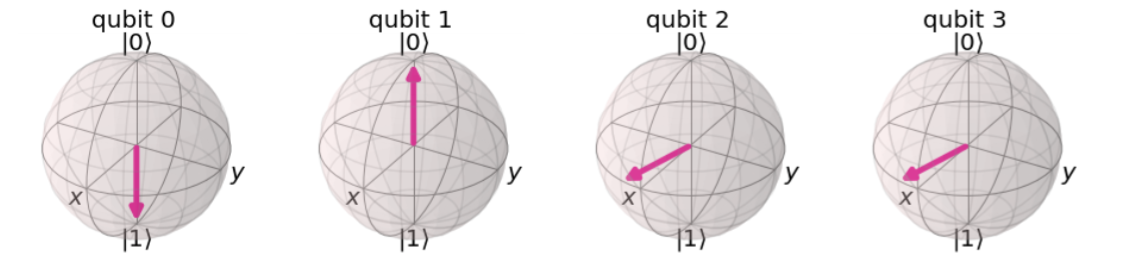
\includegraphics[width=\textwidth]{lab3/teleportBloch.png}
    \caption{teleportBloch}
    \label{fig:teleportBloch}
\end{figure}

To verify the robustness of this design, the circuit was built using IBMs remote quantum computer. The result from which can be seen in Figure \ref{fig:ibmTeleport}
\begin{figure}[h]
    \centering
    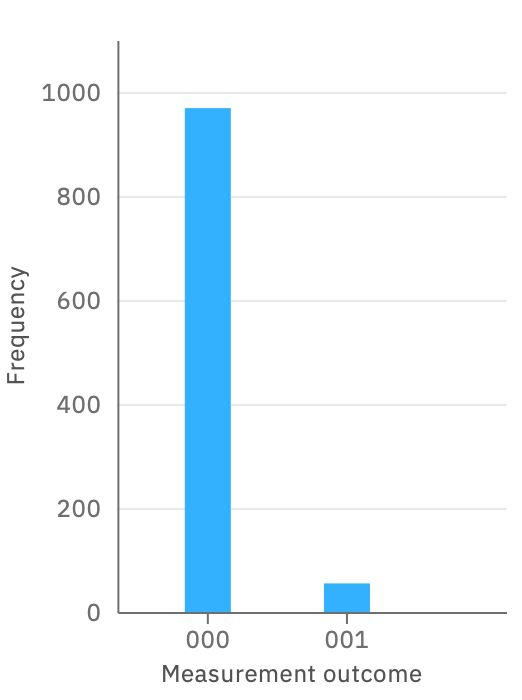
\includegraphics[width=0.38\textwidth]{lab3/ibmTeleport.png}
    \caption{ibmTeleport}
    \label{fig:ibmTeleport}
\end{figure}

\section{Comparison of results with theory}
\section{Discussion}
\textbf{Question 1:}

Follow the steps above, and the knowlege of qiskit you now have from Lab 2 to create an entanglement protocol. You may also benefit from the little revision above which introduce a couple of new features of qiskit

\textbf{Question 2:}

\textbf{2(a)}: Use IBM composer and compare its results to what you obtained above. Are they different? How so?

\textbf{2(b):} Now that you have implemented it, what could quantum telleortation be used for and why is it important?

\section{Conclusions}

\end{document}